	\chapter{Introduzione al problema}
		Da diversi anni ormai viene studiato da biologi di tutto il mondo l'affascinante comportamento della \textit{Cerithidea decollata}, comunemente chiamata \textbf{chiocciola delle mangrovie} (dall'inglese, \textit{truncated mangrove snail}).\\
		Questo particolare tipo di chiocciole ha sviluppato la capacità, a causa dell'ambiente nel quale vive, di prevedere l'altezza della marea a distanza di diverse ore, così da poter salire sul tronco di un albero e non rimanere sott'acqua.
		
		\section{Marea}
			
			La marea è un moto periodico di masse d'acqua che si innalzano e si abbassano (rispettivamente alta e bassa marea).\\
			Il fenomeno delle maree è provocato, principalmente, dalla combinazione di due fattori:
			\begin{itemize}
				\item l'attrazione esercitata sulla Terra da parte della Luna e del Sole;
				\item la forza centrifuga della rotazione del sistema Terra-Luna attorno al proprio centro di massa.
			\end{itemize}
			L'altezza raggiunta dalla marea e la sua frequenza dipendono strettamente dal luogo e dal periodo dell'anno. In generale si hanno due picchi di alta marea e due riflussi di bassa marea ogni giorno.\\
			Per gli studi effettuati in questo documento è stata utilizzata una formula in funzione del tempo (espresso in ore, come riportato di seguito) che approssima la funzione di marea:
			\[f(t) = Aa \cos \left(\frac{2 \pi t}{Ta}\right) + Ab \cos \left(\frac{2 \pi t}{Tb}\right) - D \sin \left(\frac{\pi t}{Tm} - \frac{\pi}{4}\right)\]
			assegnando ai parametri presenti i seguenti valori
			\begin{itemize}
				\item \( Aa = 1.06 \)
				\item \( Ab = 0.65 \)
				\item \( D = 0.15 \)
				\item \( Ta = 12.42 \)
				\item \( Tb = 12 \)
				\item \( Tm = 12.21 \)
			\end{itemize}
			Con questa approssimazione la marea risulta avere un periodo totale di circa 28 giorni.
			\begin{figure}[h]
				\centering
				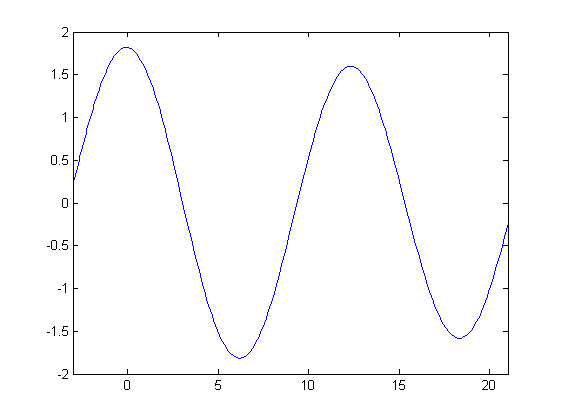
\includegraphics[width=0.8\textwidth]{tide_one_day.png}
				\caption{La funzione di marea in una giornata}
			\end{figure}
			\begin{figure}[h]
				\centering
				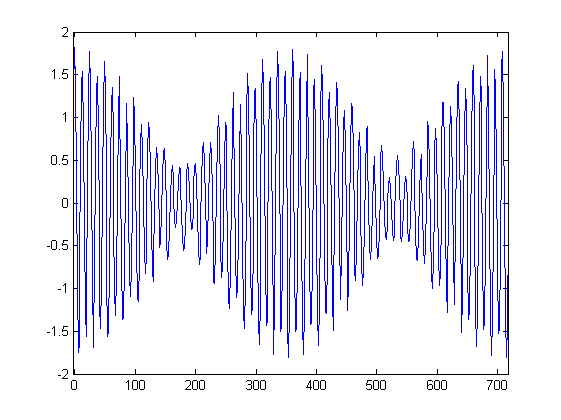
\includegraphics[width=0.8\textwidth]{tide_one_month.png}
				\caption{La funzione di marea in un mese}
			\end{figure}
			\FloatBarrier
			
		\section{Cerithidea decollata}
		
			La \textit{Cerithidea decollata}, comunemente chiamata \textbf{chiocciola delle mangrovie} (dall'inglese \textit{truncated mangrove snail}), è una specie di chiocciola di mare, ovvero un mollusco gasteropodo della famiglia delle \textit{Potamididae}.\\
			\begin{wrapfigure}{r}{0.3\textwidth}
				\centering
				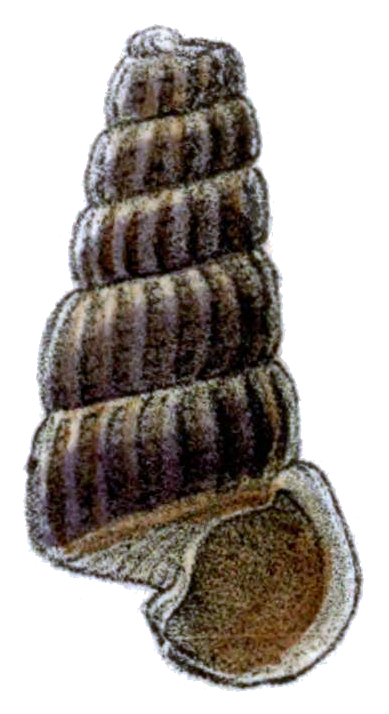
\includegraphics[width=0.3\textwidth]{shell.png}
			\end{wrapfigure}
			Gli esemplari adulti hanno una conchiglia lunga circa 3 cm composta da 5 spire, solitamente dalla punta spezzata, con circa 20 nervature per ogni spira.\\
			Queste chiocciole proliferano nelle mangrovie costiere, in particolare nella parte occidentale di Kenia, Tanzania, Mozambico, Sud Africa e Madagascar.\\
			La \textit{Cerithidea decollata} si nutre principalmente di detriti organici e di alghe portate dalla marea. Per questo vivono principalmente in piani mesolitorali (zone del litorale che dipendono dalla marea) che presentano due picchi di alta marea e due riflussi di bassa marea ogni giorno.\\
			Ogni volta che la marea si abbassa, queste chiocciole scendono al suolo per potersi nutrire. Quindi, una o due ore prima dell'innalzamento della marea, iniziano a salire sul tronco degli alberi, per poi fermarsi dai 20 ai 60 cm sopra al livello della marea futura, aspettando che questa arrivi e si abbassi di nuovo.\\
			Questo comportamento permette loro di evitare sfavorevoli effetti fisiologici legati all'immersione e sfuggire a predatori marini come granchi.\\
			È stato scoperto che queste chiocciole calcolano la propria altitudine misurando l'energia impiegata per salire: infatti, se caricate artificialmente con dei pesi, queste chiocciole salgono molto meno, credendo di essere già arrivate a destinazione.\\
			Non è ancora chiaro,tuttavia, come queste chiocciole possano prevedere l'imminente altezza di marea: la differenza del peso corporeo, dovuto alle fluttuazioni gravitazionali che causano la marea, risulta essere troppo piccola per essere rilevata da un organismo di quelle dimensioni. Si pensa che abbiano una sorta di orologio interno, combinato con l'identificazione di un qualche tipo di evento precedente alla marea, come il rilascio di acido solfidrico dal terreno, il riconoscimento degli infrasuoni prodotti dalle onde o anche le vibrazioni causate dalla cosiddetta \textit{marea di terra}.\\
			\\
			In questo studio non ci soffermeremo su come possa la \textit{Cerithidea decollata} predire effettivamente l'altezza delle maree, ma solo su quale sia la minima rete neurale necessaria per eseguire tale predizione, sia in un ambiente privo di errori che in un ambiente in cui i dati sensoriali possono essere soggetti ad errori.\\
			Quindi, per semplicità, assumeremo che queste chiocciole siano in grado di osservare, ad intervalli prefissati, il livello attuale del mare ed in base alle informazioni ottenute predire il livello della marea dopo un numero fissato di ore.
			\begin{figure}[h]
				\begin{center}
					\setlength\fboxsep{0pt}
					\setlength\fboxrule{2pt}
					\fbox{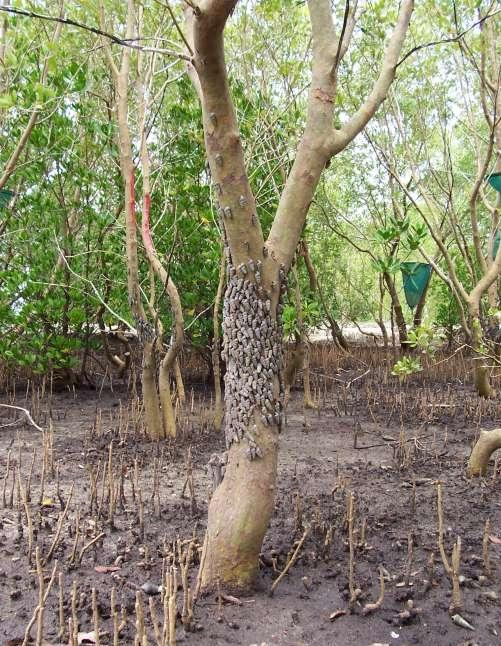
\includegraphics[width=0.8\textwidth]{tree.jpg}}
				\end{center}
				\caption{Un gruppo di \textit{Cerithidea decollata} aggrappate al tronco di un albero, in attesa della marea}
			\end{figure}